\subsection{Architecture}
Modeling the architecture of a system that supports customization of SaaS product user interfaces is not a trivial task. Most of the time, user interface design serves only one product. However, the goal of \ac{SDS} is to find common ground for multiple products in one domain. \\
Design systems define a common place where the company's products can align. Why is it impossible to develop a central system to create a common idea for user-friendly SaaS products? Not only do well-designed components help align, but a design system foundation with guidelines and principles helps developers and designers create a good product. \\

Discovering ten different design systems from popular SaaS products, as well as design systems with a common purpose, help model a new design system. The goal is to identify best practices from the SaaS world and understand the needs of companies using design systems. Table \ref{tab:design_systems_in_the_wild} reflects the idea of a design system for any business or purpose. The idea varies from design system to design system. \\
\begin{table}[!ht]
\begin{tabular}{|p{0.2\linewidth} | p{0.7\linewidth}|}
\hline
 \textbf{Name} & \textbf{Description} \\ \hline
ServiceNow \cite{servicenow_servicenow_nodate}  & Platform design system.  Guidance to create components and upload them to the platform. \\ \hline
Adobe Spectrum  \cite{spectrum_adobe_spectrum_nodate} & User centralised design system. Many well designed components with matching guide to deliver a great experience. Built in web components and react components. \\ \hline
Zendesk Garden \cite{zendesk_garden_zendesk_nodate} & Basic design system with guidelines, components and patterns. Tailwindcss integration. Built in react components. \\ \hline
Atlassian Design System \cite{atlassian_design_system_atlassian_nodate} & Design System connected with company values. A lot of guides on how to use designs, components and to write content. Includes also employee motivation. Built in react components. \\ \hline
Base Web  \cite{base_base_nodate} & Open source design system. Used by Uber. Providing a blog and guides on how to use the base design system. Design System intended to be used as baseline and should be overwritten when used. No principles or values included. \\ \hline
SAP Fiori  \cite{sap_fiori_nodate} & Standard design system. Focus on accessibility and multiple device support. Including many themes for different applications. Delivers a toolkit to better use the design system as a designer.  \\ \hline
GOV UK Design System  \cite{govuk_govuk_nodate} & Not really a design system. Missing guidelines and principles. Externals can propose changes. Providing CSS classes for HTML elements.  \\ \hline
Lightning Design System \cite{lightning_design_system_lightning_nodate} & Design System to support developers and designer at their work. 4 principles with a clear message to align every user. Guidelines and best practices on many topics.  Components are built with pure CSS classes. \\ \hline
Google Matrial Design \cite{google_material_2022} & Open source design system. Providing the user with design principles which helps to understand the usage of the design system. Material Design provides only components and no patterns. Blogs and further resources are helping additionally to the guidelines. Components are built with pure CSS classes. \\ \hline
Pluralslight Design System \cite{pluralsight_ds_nodate} & Design System without principles and guidelines. For the moment only components are present. Providing a workflow for developers and designers to contribute to the design system.  Only few patterns. Built with react components.  \\ \hline
\end{tabular}
\caption{\label{tab:design_systems_in_the_wild} Overview of 10 existing design systems}
\end{table}

A good reference for a design system with a suitable use case is the Base Web Design System. Its purpose of providing a base of styles and functional components helps developers to extend the design system and create their own for their products. Also, the fact that this design system is open source underlines that the community is developing this design system, not a corporate design team. As a shared design system, it focuses particularly on accessibility and internationalization. The tutorial explains how to extend and use the design system, which is a perfect reference model for \ac{SDS}. \\

But there are also disadvantages. The Base Web Design System lacks guidelines and principles that are crucial for a design system.
A look at Google's Material Design shows that even an open-source and versatile design system can have design principles. Design principles help developers get an idea of how to develop and design with the system. Therefore, design principles are essential for design systems. \\

Another reason why the Base Web Design System is not a perfect model is the use of React to create the components. The design system forces developers to use React as a front-end library in their products. This is not an option for SDS to bind developers to a single front-end framework. Therefore, this characteristic of the Base Web Design System is unsuitable. Other examples such as the GOV UK Design System or Salesforce's Lightning Design System show that it is possible to create components using only web standards. \\

With these requirements, Figure \ref{architecture_sds} draws an example architecture of what the SDS may look like.\\
\begin{figure}[htbp]
\centerline{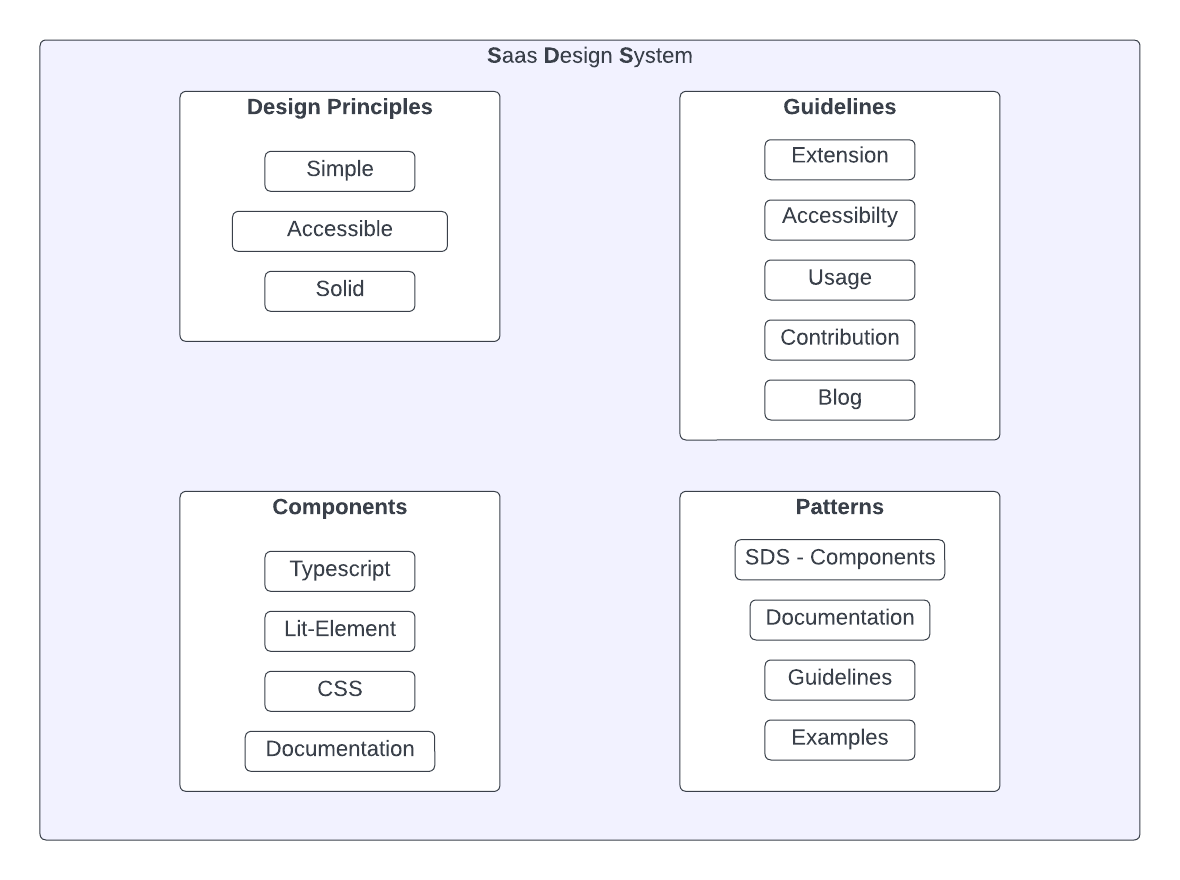
\includegraphics[width=\linewidth]{images/architecture_sds.png}}
\caption{Architecture of SaaS Design System}
\label{architecture_sds}
\end{figure}

The architecture model shown above divides the \acl{SDS} into four parts. The details of these parts are explained in the next sections.
\subsubsection{Design Principles}
In terms of design principles, the \ac{SDS} strives to keep them lean and easy to understand. This helps the design system to serve as a basis for other design systems. \\

The \textbf{Simple} principle states that component design should not have unnecessary styles or features that make it difficult to extend. This principle underlines the idea of keeping the entire design system lean. Developers understand lean descriptions and clear documentation much better than reading a wall of text. \\

Many products strive to implement accessibility in their products. With the \textbf{Accessible} principle, \ac{SDS} emphasizes the importance of accessible user interfaces. This emphasizes not only significant in terms of inclusion, but also helps accessibility in the overall user experience for all users. Because \textbf{Accessibility} doesn't just come into play when it relates to disabilities, it helps the application with the overall user experience. \\

The third and final principle is \textbf{Solid}. As stated earlier, the \ac{SDS} is a foundation for other design systems to build upon. Therefore, the importance of a stable and consistent API is paramount. Components and patterns should not change regularly. Versioning allows developers to choose their desired version of the \ac{SDS} without having to adapt. For this reason, the design system has deliberately chosen \textbf{Solid} as the third and final principle. \\

The first iteration of the \acl{SDS} principles provides a good foundation on which to build. As described in Chapter \ref{design_principles}, finding the right design principles will take a few iterations to get right. But by starting with \textbf{Simple}, \textbf{Accessible}, and \textbf{Solid}, designers and developers will find the right way to use this design system.
\subsubsection{Guidelines}
The design principles just presented form the basis for the \ac{SDS} guidelines. In addition to the core guidelines on extension, accessibility, and essential use, some guidelines focus on contributions and collaboration. As this is an open-source system, as many people as possible should be able to work on it. \\

The extension guidelines address how to integrate \ac{SDS} as the basis for a company's own design system. It shows developers and designers how to create their own from the components provided. The goal of such a guide is to help system developers use the SDS as a foundation. The guide helps developers and designers to build their system on the SDS instead of introducing complex integrations. \\

Since accessibility is also a design principle, a guideline must define what the \ac{SDS} means by accessibility. The guideline should give the user a definition and sources for accessibility. But there should also be a manual for self-designed components to help users implement accessibility. Understanding this guide, users should no longer have accessibility questions when designing new interfaces. \\

As a third guideline, the \ac{SDS} will support the user in using the system. This guide could also be seen as an entry guide and will cover the basics. Importing the design system, proper bootstrapping, and guidance on configuring the system. Such a guideline may seem self-explanatory, but the lack of it often prevents users from using the system. The usage guide should be as simple as possible and cover every small step needed to get started with the \ac{SDS}. \\

One goal of this design system is to be developed by the community for the community. However, this can quickly get out of hand if everyone contributes without guidance. Therefore, it is crucial to introduce some from the beginning. This guide guides how to contribute to the component library and enforce changes to the guidelines and principles. \\
As this design system evolves over time, there should be opportunities to change and adapt. What this will look like in the end will evolve over time. What this will look like in the end will evolve. Some ideas could be a voting process or an RFC process, as is standard in the software industry. \\


Some design systems introduce blogs and forums for knowledge exchange to achieve high interactivity in a design system. In this way, users can connect, discuss and contribute to ideas to further improve the design system. A well-moderated blog and forum will further enhance the community around the \ac{SDS}. \\
Since the \ac{SDS} won't be a product but an open source project, forums and blogs will be the marketing platform to spread the idea of the design system. The goal is to build a strong community around the \ac{SDS}. So that some of the advocates end up contributing to the actual design system. \\

In summary, the guidelines of the \acl{SDS} are about creating a community around the design system. Developer and designers should not only using it for their desired goal, but see the potential to collaborate for the bigger picture behind \ac{SDS}.


\subsubsection{Components} \label{sds-component}
Without well-assembled components, design systems cannot exist. Therefore, choosing the right technology package for building components is very important. In the case of \ac{SDS}, one of the most essential requirements is that the system is usable independently of the frontend framework used. To achieve this, \ac{SDS} uses the web components supported in almost all modern browsers. As it is possible to create web components without importing libraries or frameworks, it is for \ac{SDS}. \citep{mdn_web_component_nodate} \\

Creating web components natively can be complicated. The Lit Element framework helps developers build web components by eliminating some of the pitfalls of implementing web components from scratch. With a focus on ease of understanding, intelligent DOM updates, and a small package size (5 KB), Lit is a perfect addition for creating components for design systems based on standard web components. \citep{lit_nodate} \\

To further assist developers, \ac{SDS} uses Typescript, a superset of Javascript. It extends Javascript with types and interfaces. Typescript must be compiled into Javascript for the browser to understand, but this allows the developer to find errors much faster because it fails at compile time rather than at runtime. \citep{microsoft_typescript_nodate} \\

The \ac{SDS} uses custom CSS variables to use and provide design tokens for colors or spacing. The design system imports the design tokens into the root element during bootstrapping. In the documentation of the design system exists a page with an overview of all design tokens. \citep{mdn_css_vars_nodate} \\

Last but not least, users must have access to the documentation of the components and tokens. Storybook is the documentation tool for the \ac{SDS}. It has many built-in functions that are useful for documenting components. With MDX, the combination of Markdown templating (MD) and code injection via JSX, it is possible to write fluid documentation without having to jump back and forth between files while documenting components. \citep{otander_markdown_2017} \\

With this technology stack, \ac{SDS} provides users with highly reusable web components that are easy for users to access but also easy for contributors to develop.


\subsubsection{Patterns}
An essential part of a design systems are patterns. Patterns try to combine the capabilities of a design system with the design of user interfaces. In the case of \ac{SDS}, patterns help developers automatically apply best practices and web standards without having to read an entire text. \\

The combination of standard HTML elements and components from SDS creates patterns in the SDS. These are easily accessible to the developer by copying and pasting code into the desired application that has implemented the SDS. Additional documentation helps the developer to avoid using patterns where they do not belong. \\

SDS patterns come with special documentation that allows for customization and redesign. The documentation enables developers to fulfill their requirements for their own design system.\\

As with the component documentation, live examples show the developer how the design system patterns will work in the final product. Several different examples for each pattern present the possibilities for individual design. \ac{SDS} users have the opportunity to share their creations and application of patterns below the documentation. \\

The big benefit of using SDS is the patterns. They simplify web accessibility compliance and leave enough room for individual user designs. The correct use of patterns is crucial for a successful integration of \ac{SDS} into a product.
